\documentclass[12pt, a4paper]{article}

\usepackage{array}
\usepackage[portuguese]{babel}
\usepackage{float}
\usepackage[a4paper, margin=2cm]{geometry}
\usepackage{graphicx}
\usepackage{hyperref}
\usepackage{pdfpages}
\usepackage{setspace}

\title{\textbf{Interface Pessoa-Máquina \\ \large Trabalho Prático -- Fase I}}
\date{16 de março de 2025}
\author{Grupo 12 \\
    \url{https://www.figma.com/design/Ps4VLCPz66bKq5p2ypzrDR/Projeto-IPM}}

\begin{document}

\begin{center}
    
\includegraphics[width=0.25\textwidth]{res/cover/school-of-engineering.eps}
\end{center}

{\let\newpage\relax\maketitle}
\maketitle
\thispagestyle{empty}

\chardef\_=`_
\onehalfspacing
\setlength{\parskip}{\baselineskip}
\setlength{\intextsep}{2\baselineskip}
\setlength\belowcaptionskip{-\baselineskip}
\setlength{\parindent}{0pt}
\def\arraystretch{1.5}

\vspace{2cm}
\begin{center}
    \begin{tabular}{>{\centering}p{0.25\textwidth}
                    >{\centering}p{0.25\textwidth}
                    >{\centering\arraybackslash}p{0.25\textwidth}}
        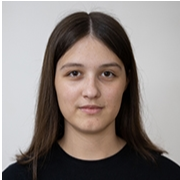
\includegraphics[width=3.5cm]{res/cover/A104437.png} &
        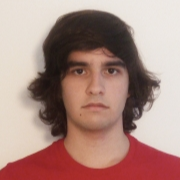
\includegraphics[width=3.5cm]{res/cover/A104348.png} &
        
\includegraphics[width=3.5cm]{res/cover/A104263.png}  \\

        Ana Oliveira & Humberto Gomes & Inês Marques \\
        A104437      & A104348        & A104263
    \end{tabular}

    \begin{tabular}{>{\centering}p{0.25\textwidth}
                    >{\centering\arraybackslash}p{0.25\textwidth}}
        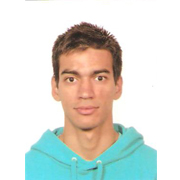
\includegraphics[width=3.5cm]{res/cover/A76350.jpg} &
        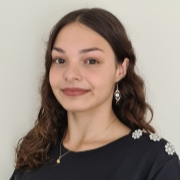
\includegraphics[width=3.5cm]{res/cover/A104179.png} \\

        Rafael Vilas Boas & Sara Lopes \\
        A76350            & A104179
    \end{tabular}
\end{center}

\begin{abstract}
    \noindent
    No âmbito deste trabalho prático, foi prototipada uma interface de utilizador de um sistema para
    a gestão de horários de um curso universitário, utilizado tanto pelos alunos como pelo diretor
    de curso. Neste documento, apresenta-se a interface modelada com recurso à ferramenta Figma
    \cite{figma}, justificando as várias decisões tomadas face aos perfis dos utilizadores da
    aplicação. Perante o grande volume de dados que são horários, o principal foco do
    desenvolvimento desta interface foi a apresentação desta informação de uma forma familiar,
    flexível, e sem sobrecarregar o utilizador. Foi também realizada uma avaliação da interface
    apresentada, fazendo uso das heurísticas de Nielsen \cite{nielsen}. Apesar de algumas limitações
    da ferramenta de modelação, julga-se ter construído um protótipo de uma interface que cumpre os
    objetivos do enunciado, e que se encontra suficientemente detalhado para a sua implementação.
\end{abstract}

\section{Análise da Interface Desenvolvida}

\subsection{Página ``Iniciar Sessão''}

A primeira página construída foi a página de início de sessão, que é apresentada ao utilizador
quando este abre a aplicação. Nesta página, tal como descrito nos cenários 1 e 4, tanto o diretor
de curso como as alunos inserem as suas credenciais para se autenticarem:

\begin{figure}[H]
    \centering
    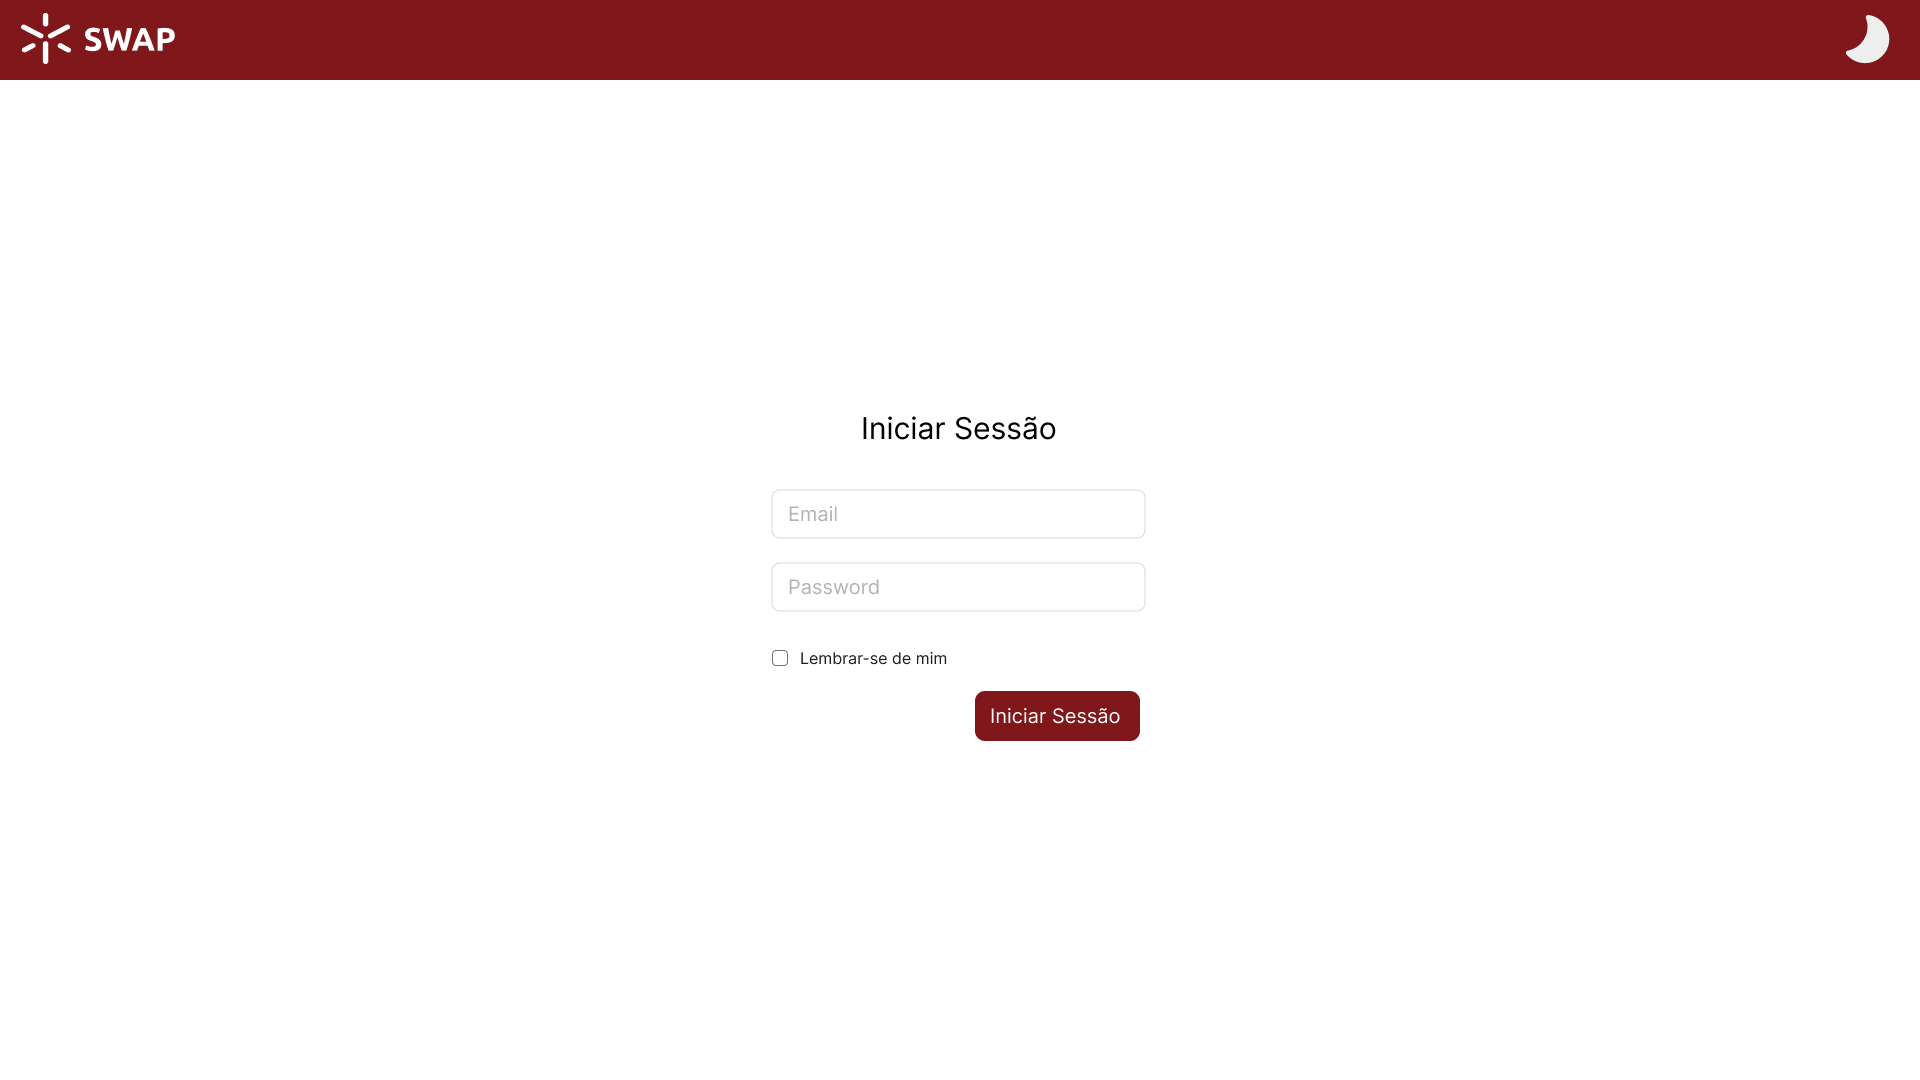
\includegraphics[width=0.8\textwidth]{res/prototype/iniciar-sessao.png}
    \caption{Captura de ecrã do protótipo da página ``Iniciar Sessão''.}
    \label{iniciar-sessao}
\end{figure}

Como não há nada de inovador nesta página, procurou-se inspiração em páginas de início de sessão de
diversos outros \emph{websites}, para se desenvolver uma interface consistente com o que o
utilizador já pode estar familiarizado. Logo, a página é constituída por um título, ``Iniciar
Sessão'', e dois campos de texto explicados com \emph{placeholders}, indicando que informação o
utilizador deve inserir (o seu endereço eletrónico e a sua palavra-passe).

O utilizador também pode escolher se o sistema deve ou não perguntar pelas suas credenciais de
\emph{login} no próximo acesso à aplicação. Caso se opte que o sistema se ``lembre do utilizador'',
é possível poupar algum tempo em usos futuros e recorrentes da aplicação, algo especialmente
importante para o perfil do diretor de curso, que deseja minimizar o seu tempo gasto na gestão de
horários. No entanto, por motivos de segurança, por exemplo, quando a aplicação é utilizada num
computador partilhado, deverá ser possível impedir que o sistema permita o acesso a utilizadores
antes deles providenciarem as suas credenciais.

O perfil da Maria corresponde ao de uma aluna de informática. Apesar de não constar no enunciado, é
de conhecimento geral que muitos dos alunos deste curso não apreciam interfaces em tons claros. Por
este motivo, procurando desenvolver-se uma interface customizável, também se prototipou uma variante
desta interface em tons escuros, que se apresenta abaixo:

\begin{figure}[H]
    \centering
    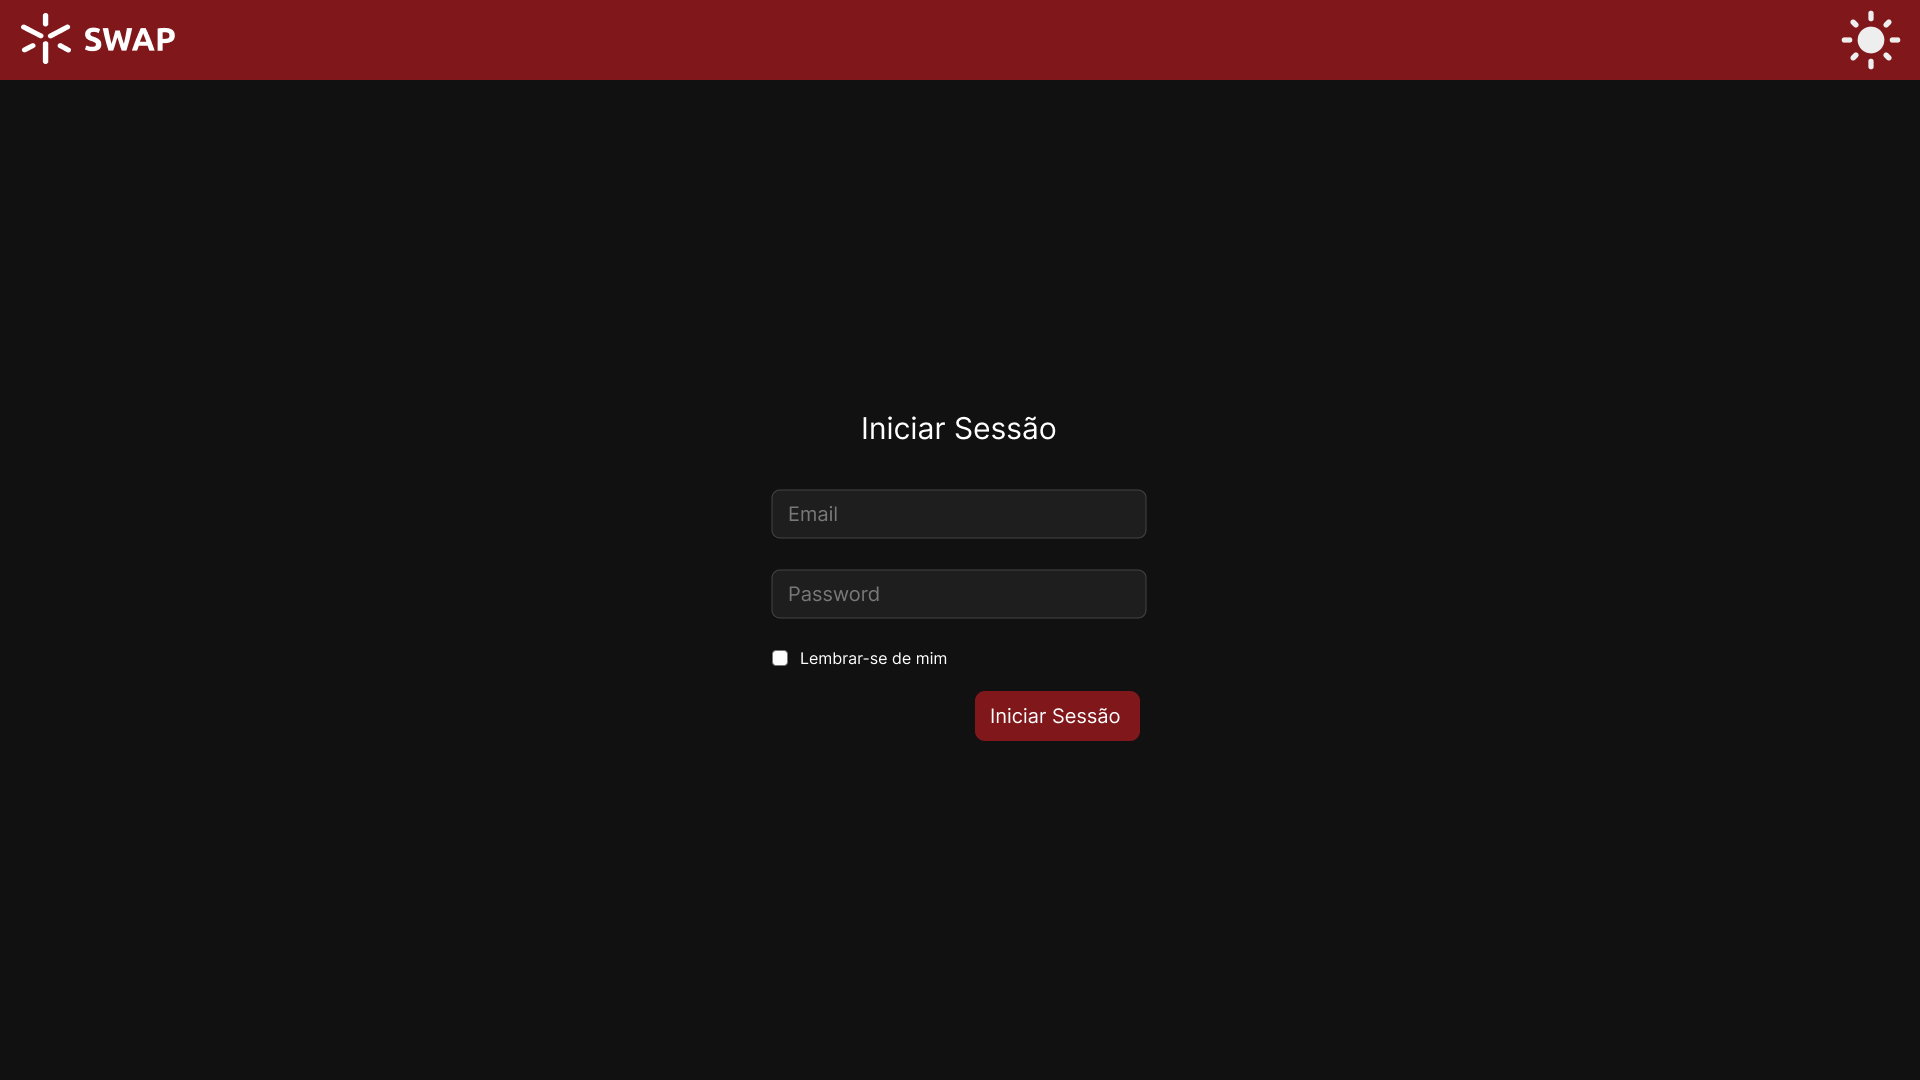
\includegraphics[width=0.8\textwidth]{res/prototype/iniciar-sessao-dark.png}
    \caption{Captura de ecrã do protótipo da página ``Iniciar Sessão'' no tema escuro.}
    \label{iniciar-sessao-dark}
\end{figure}

Visto que o objetivo deste trabalho prático é a prototipagem da estrutura e da funcionalidade da
interface, e não da sua aparência, apenas se prototipou esta página em modo escuro. Para alternar
entre estes dois estilos da aplicação, está sempre disponível um ícone na barra de navegação, uma
lua para ir de modo claro para modo escuro, e um sol para o inverso. Para indicar que é possível
clicar nestes ícones, o seu tom muda quando o utilizador move o cursor para cima dos mesmos. Apesar
de se ter utilizado uma iconografia presente em diversas outras interfaces, Material Icons
\cite{material-icons}, após sobrevoar um ícone com o cursor por algum tempo, uma \emph{tooltip} deve
aparecer, descrevendo o ícone em palavras ao utilizador. Devido a limitações do Figma, não foi
possível prototipar esta funcionalidade. Porém, segue, abaixo, uma simulação visual da aparência
desta \emph{tooltip}:

\begin{figure}[H]
    \centering
    
\includegraphics[width=0.3\textwidth]{res/prototype/icon-tooltip.png}
    \caption{\emph{Tooltip} sobre o ícone de mudança para o tema escuro.}
    \label{icon-tooltip}
\end{figure}

\subsection{Página ``O meu Horário''}

Caso seja um aluno a iniciar sessão, será redirecionado para a página ``O meu Horário'', onde o seu
horário lhe é apresentado, como descreve o cenário 4. Tendo em conta o perfil da utilizadora Maria,
como esta é estudante, assume-se que ela precise de consultar esta página com frequência: para saber
para que sala se deve dirigir no fim de uma aula, que cadernos deve levar na mochila para o dia
seguinte de aulas, \emph{etc.}. Por este motivo, decidiu-se que esta seria a primeira página
apresentada a um estudante depois deste iniciar sessão, pois é a que este mais provavelmente
desejará aceder. Segue-se, abaixo, o protótipo desta página:

\begin{figure}[H]
    \centering
    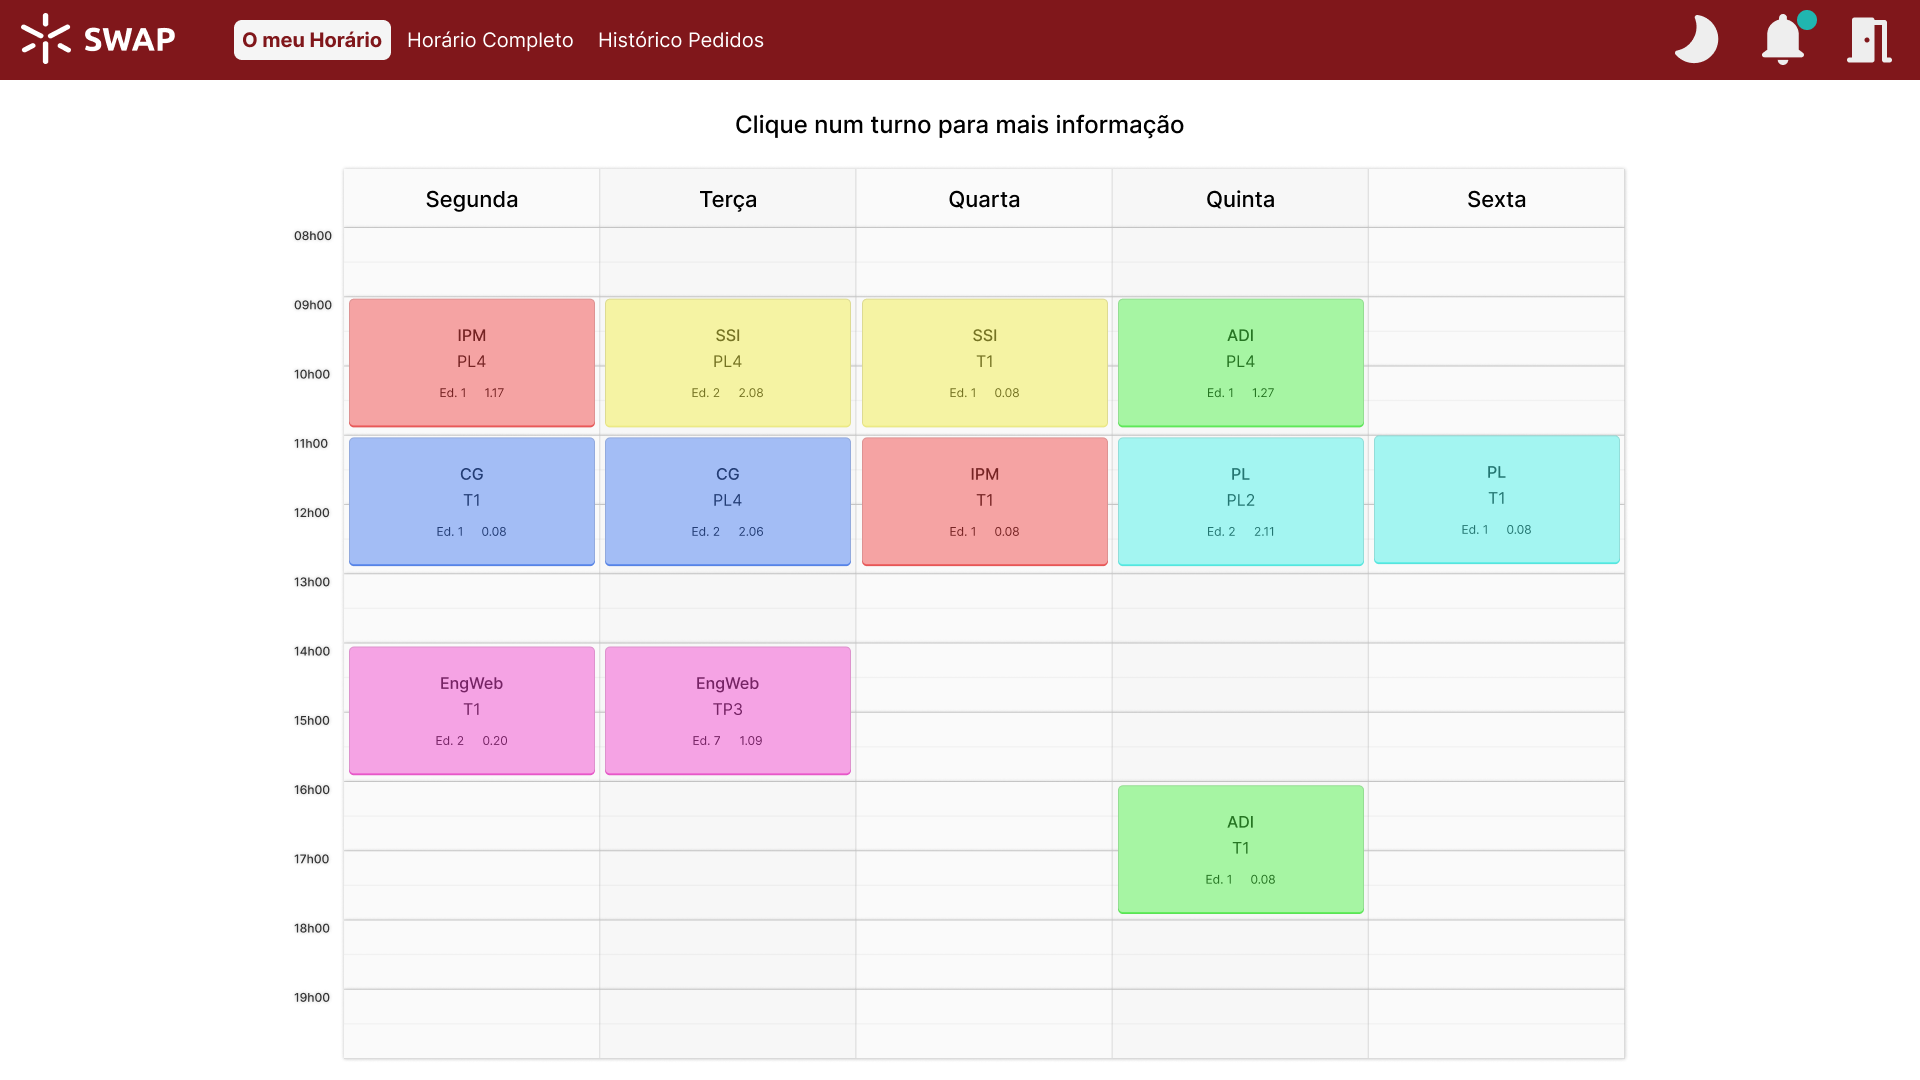
\includegraphics[width=0.8\textwidth]{res/prototype/o-meu-horario.png}
    \caption{Captura de ecrã do protótipo da página ``O meu Horário''.}
    \label{o-meu-horario}
\end{figure}

Antes de justificar a estrutura do conteúdo desta página, é importante explicar o funcionamento da
sua barra de navegação, também presente nas outras páginas às quais os estudantes podem aceder.
Depois do ícone da aplicação, segue uma lista de hiperligações para as páginas acessíveis. A página
onde o utilizador se encontra é realçada com o esquema de cores inverso ao das restantes. Deste
modo, o utilizador sabe sempre em que página se encontra. Do lado direito da barra de navegação,
surgem ícones para trocar o tema da interface (claro ou escuro), ir para a página de notificações, e
para terminar sessão. Novamente, todos estes ícones devem ter uma \emph{tooltip} associada, mesmo
que sejam semelhantes aos utilizados por interfaces de outras aplicações (para uma maior
consistência externa). Para chamar a atenção do utilizador quando há novas notificações, um círculo
surge no canto superior direito do ícone do sino.

O principal elemento do conteúdo da página ``O meu Horário'' é o horário do aluno. Para o apresentar
de uma forma familiar ao utilizador, este é representado como uma grelha de turnos, com os dias da
semana em colunas e as horas do dia em linhas. Os turnos são posicionados nesta grelha conforme a
sua localização temporal. Adicionalmente, para ser fácil que o utilizador distinga entre turnos
diferentes UCs, é associada uma cor a cada UC.

É possível clicar num turno para abrir um diálogo com mais informação. Para ser observável que esta
ação é possível, sobrevoar o cursor a um turno deve mudar a sua cor, e o ícone do cursor deve também
mudar para o do dedo indicador, como mostra a figura abaixo:

\begin{figure}[H]
    \centering
    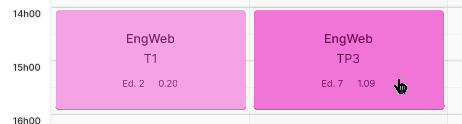
\includegraphics[width=0.6\textwidth]{res/prototype/turno-hover.png}
    \caption{Mudança de cor e de cursor com o sobrevoo do cursor a um turno.}
    \label{turno-hover}
\end{figure}

Mesmo com este efeito, alguns elementos deste grupo de trabalho, também estudantes como a Maria,
tiveram alguma dificuldade em perceber que era possível clicar nos turnos. Ademais, também não
seria possível que utilizadores a utilizar a aplicação sem um rato (por exemplo, com um ecrã tátil)
se apercebessem que era possível interagir com os turnos. Por esse motivo, o texto ``Clique num
turno para mais informação'' foi colocado no topo da página.

Quando o utilizador clica num turno, deve sobrepor-se um diálogo com informação sobre o mesmo, como
mostra a figura abaixo. O fundo da página é escurecido para realçar o diálogo, que mostra mais
detalhes sobre o turno em que o utilizador clicou, como o docente que o leciona e a sua lotação.
Para não sobrecarregar o utilizador com informação na visão normal do seu horário, esta foi colocada
neste diálogo à parte, permitindo uma observabilidade do estado do programa mesmo em ecrãs de
tamanho limitado. É possível fechar este diálogo clicando no ``X'' no seu canto superior direito, o
que é consistente com outras interfaces WIMP (\emph{Windows, Icons, Menus, Pointer}), mas também
clicando fora da sua área (na página ``atrás''), para esta ação ser mais simples para utilizadores
com problemas de destreza manual ou a utilizar ecrãs mais pequenos.

\begin{figure}[H]
    \centering
    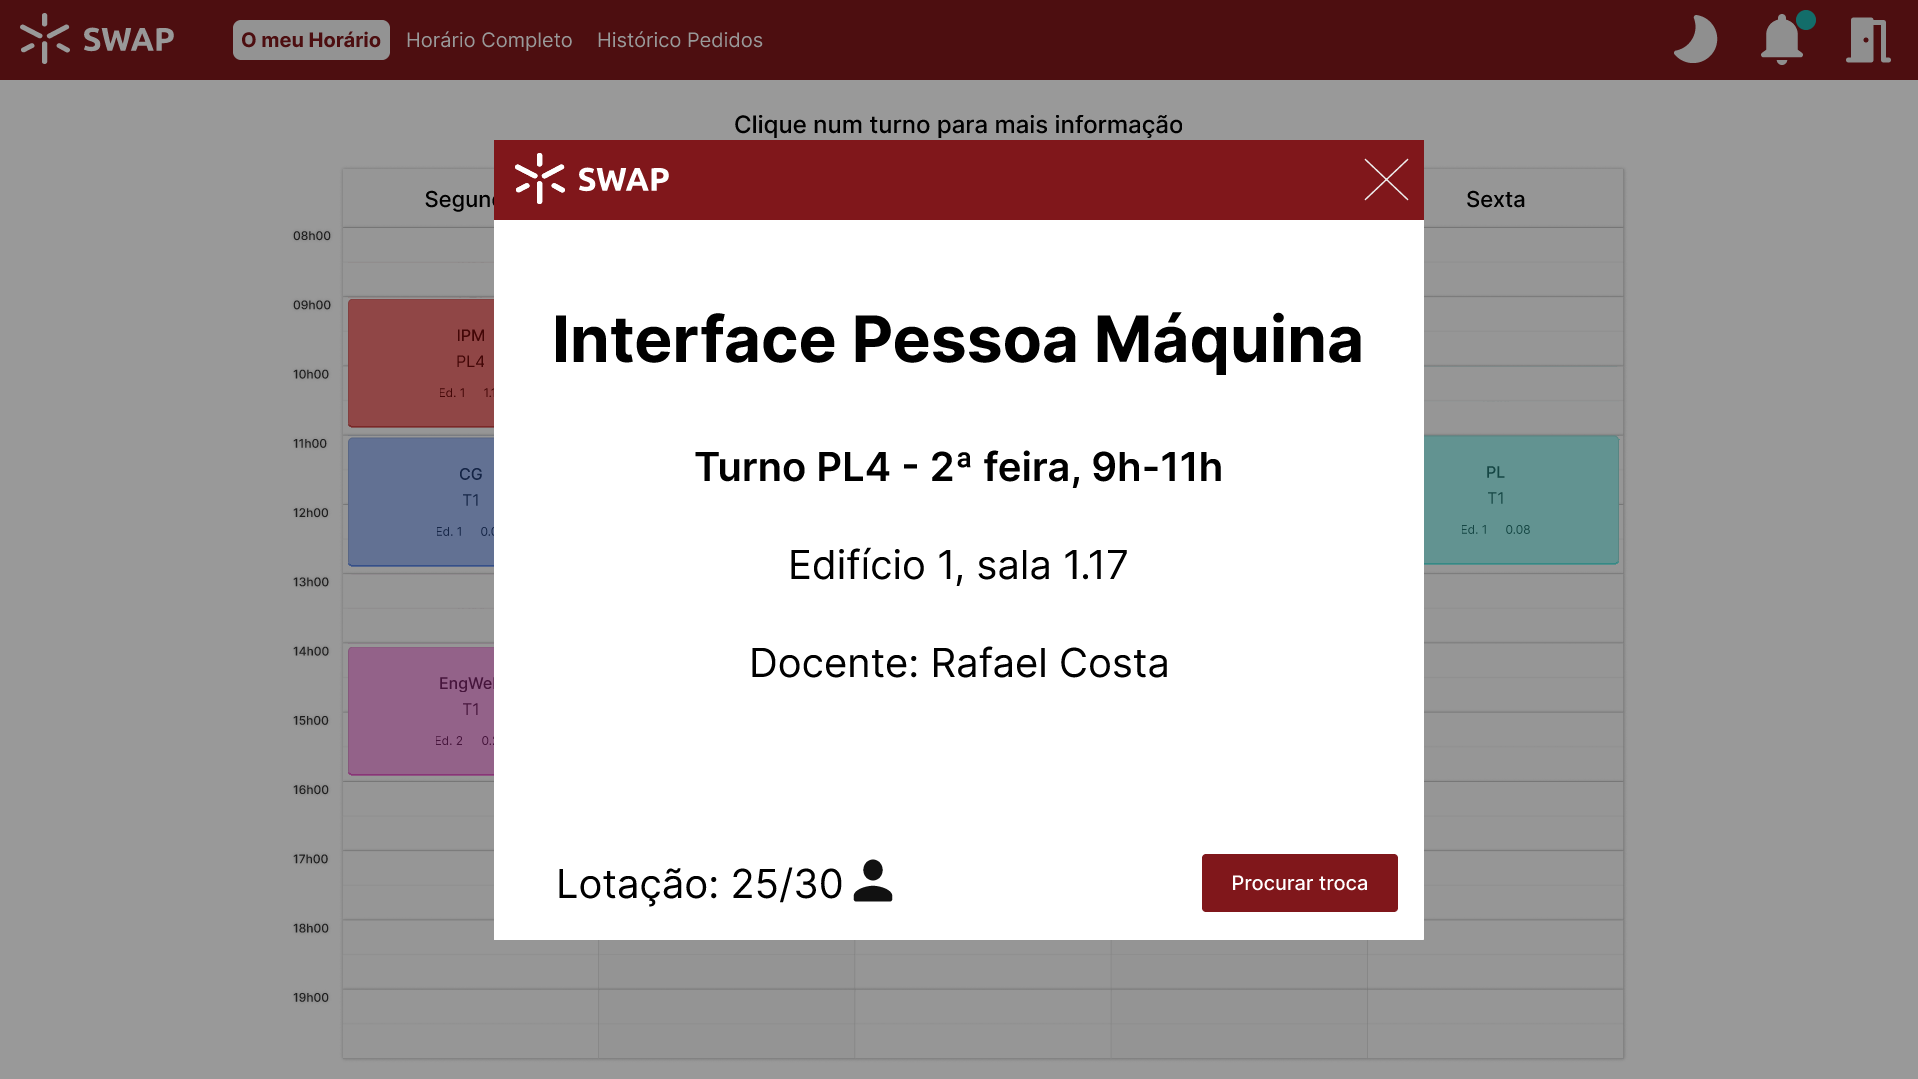
\includegraphics[width=0.6\textwidth]{res/prototype/dialogo-informacao-turno.png}
    \caption{Diálogo com informação de um turno na página ``O meu Horário''.}
    \label{dialogo-informacao-turno}
\end{figure}

A partir deste diálogo, como referido no cenário 4, é possível que o utilizador troque o turno que
selecionou, carregando no botão ``Procurar troca''. Fazê-lo deve fechar o diálogo e alterar os
conteúdos da página ``O meu Horário'' para algo como o seguinte:

\begin{figure}[H]
    \centering
    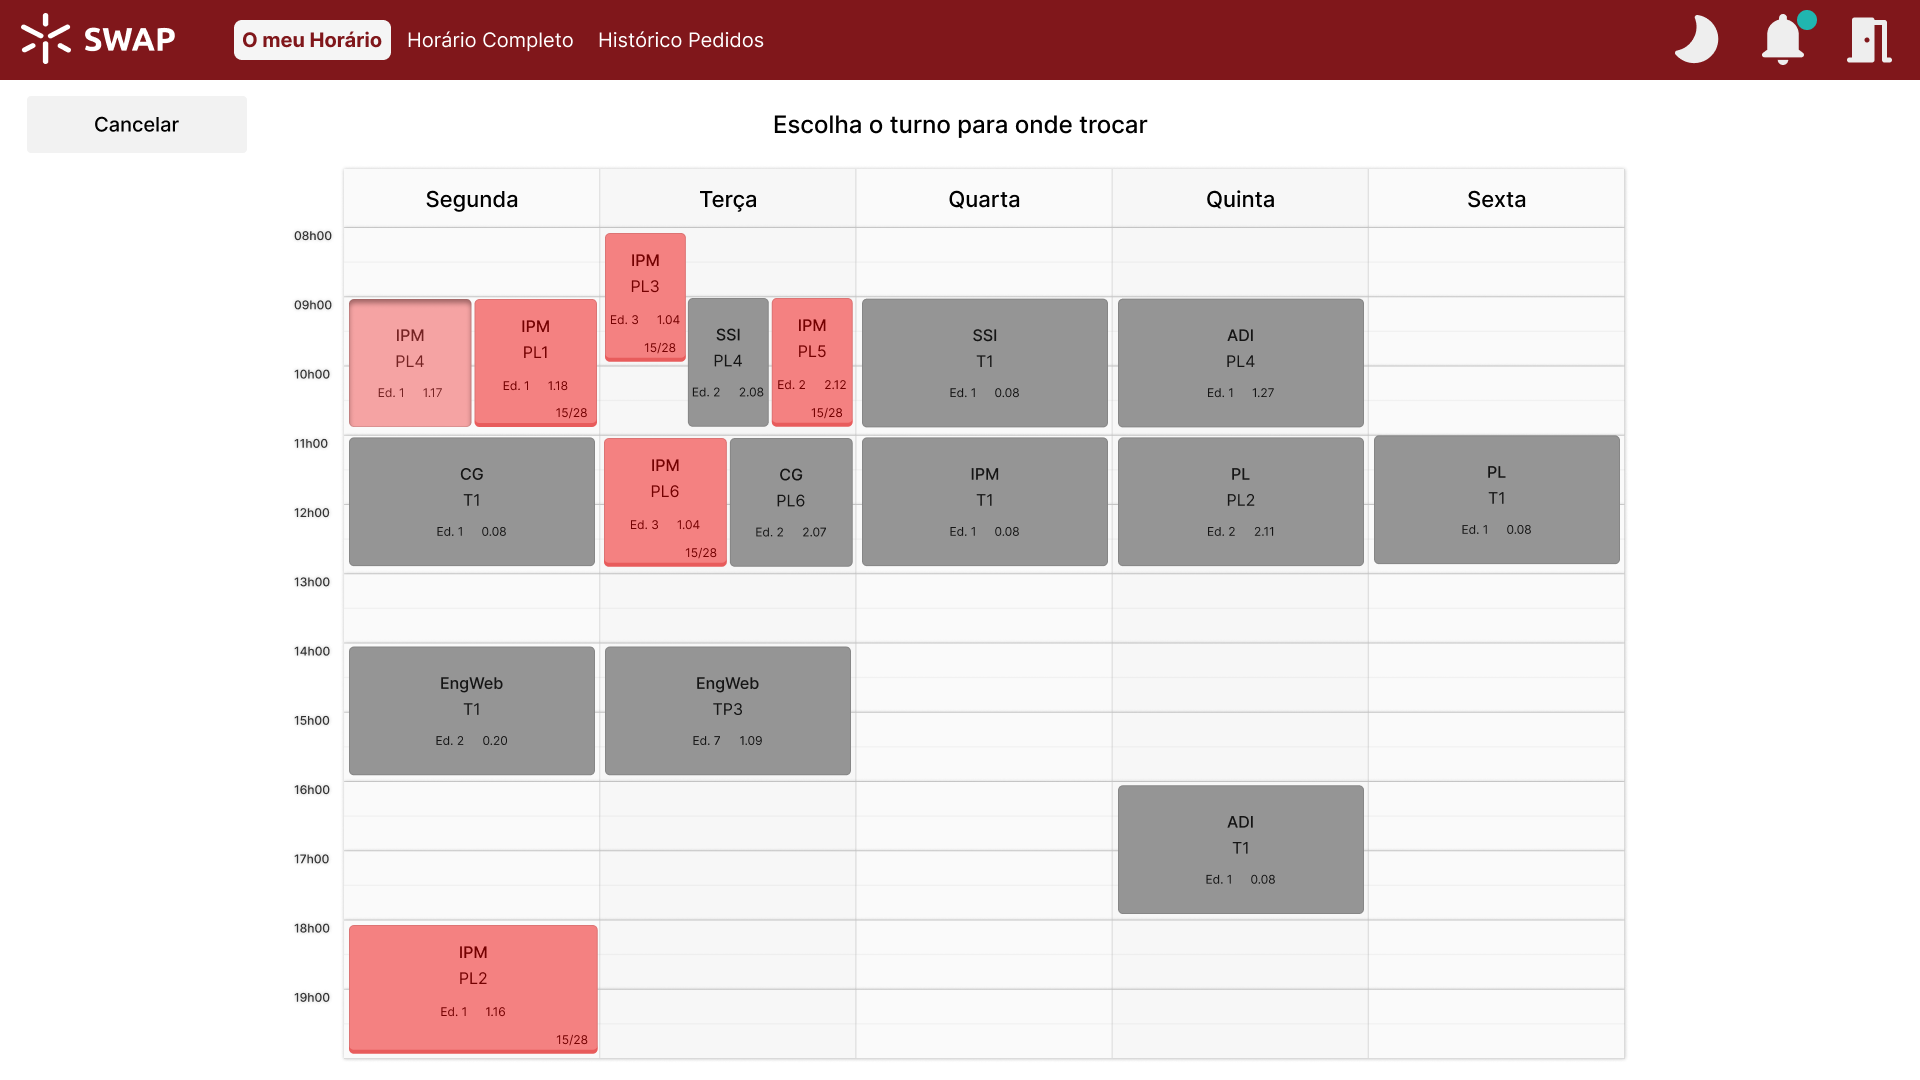
\includegraphics[width=0.8\textwidth]{res/prototype/o-meu-horario-trocar.png}
    \caption{Captura de ecrã do protótipo da página ``O meu Horário'' durante uma troca de turnos.}
    \label{o-meu-horario-trocar}
\end{figure}

Como se pode observar, os turnos em que o aluno se encontra inscrito são representados a cinzento.
Ademais, não são alterados de qualquer modo quando o cursor os sobrevoa, indicando que não é
possível interagir com eles. Por outro lado, o conjunto de turnos do mesmo tipo que o turno
selecionado (por exemplo, turnos práticos de IPM), são representados a uma cor viva, que,
juntamente com o efeito descrito na figura \ref{turno-hover}, indica que é possível interagir com
eles. Uma exceção é o turno que o utilizador pretende trocar, que é apresentado num tom entre o
cinzento e a cor viva dos restantes turnos, e sem o efeito de \emph{hover}. Deste modo, mostra-se
que não é possível trocar para este turno, mas que este turno pertence ao conjunto dos turnos
selecionados. Novamente, como o efeito de \emph{hover} não será visível para utilizadores da
aplicação com ecrãs táteis, um texto de ajuda, ``Escolha o turno para onde trocar'', é apresentado
no topo da página.

Nesta vista da página, os turnos selecionáveis pelo utilizador já apresentam a sua lotação, pois
esta informação pode ser útil para o aluno escolher para que turno deve pedir para trocar. No
entanto, é de notar que o sistema não deve impedir que um aluno envie um pedido de troca para um
turno cheio. A título de exemplo, o aluno pode ser um trabalhador estudante e o diretor de curso
colocá-lo nesse turno mesmo assim (cenário 3), ou outro aluno pode já ter enviado um pedido a
requisitar para sair desse turno. Ademais, esta interface permite facilmente ver quais as trocas de
turnos que conduzem a sobreposições, para o aluno as poder evitar. Novamente, o sistema não deve
impedir estes pedidos de troca: isso é responsabilidade do diretor de curso caso assim o deseje.

Quando o utilizador inicia o processo de troca de turno, pode aperceber-se que nenhuma opção lhe é
conveniente. Nesse caso, pode cancelar a operação carregando no botão ``Cancelar'' do lado esquerdo
da página, ou carregando na página ``O meu Horário'' na barra de navegação, reiniciando o estado
desta página e abortando a troca de turnos.

Quando se clica num turno, deve ser enviado um pedido de troca ao diretor de curso. No entanto,
como não é possível retroceder no envio deste pedido, um diálogo de confirmação deve surgir após
clicar num turno:

\begin{figure}[H]
    \centering
    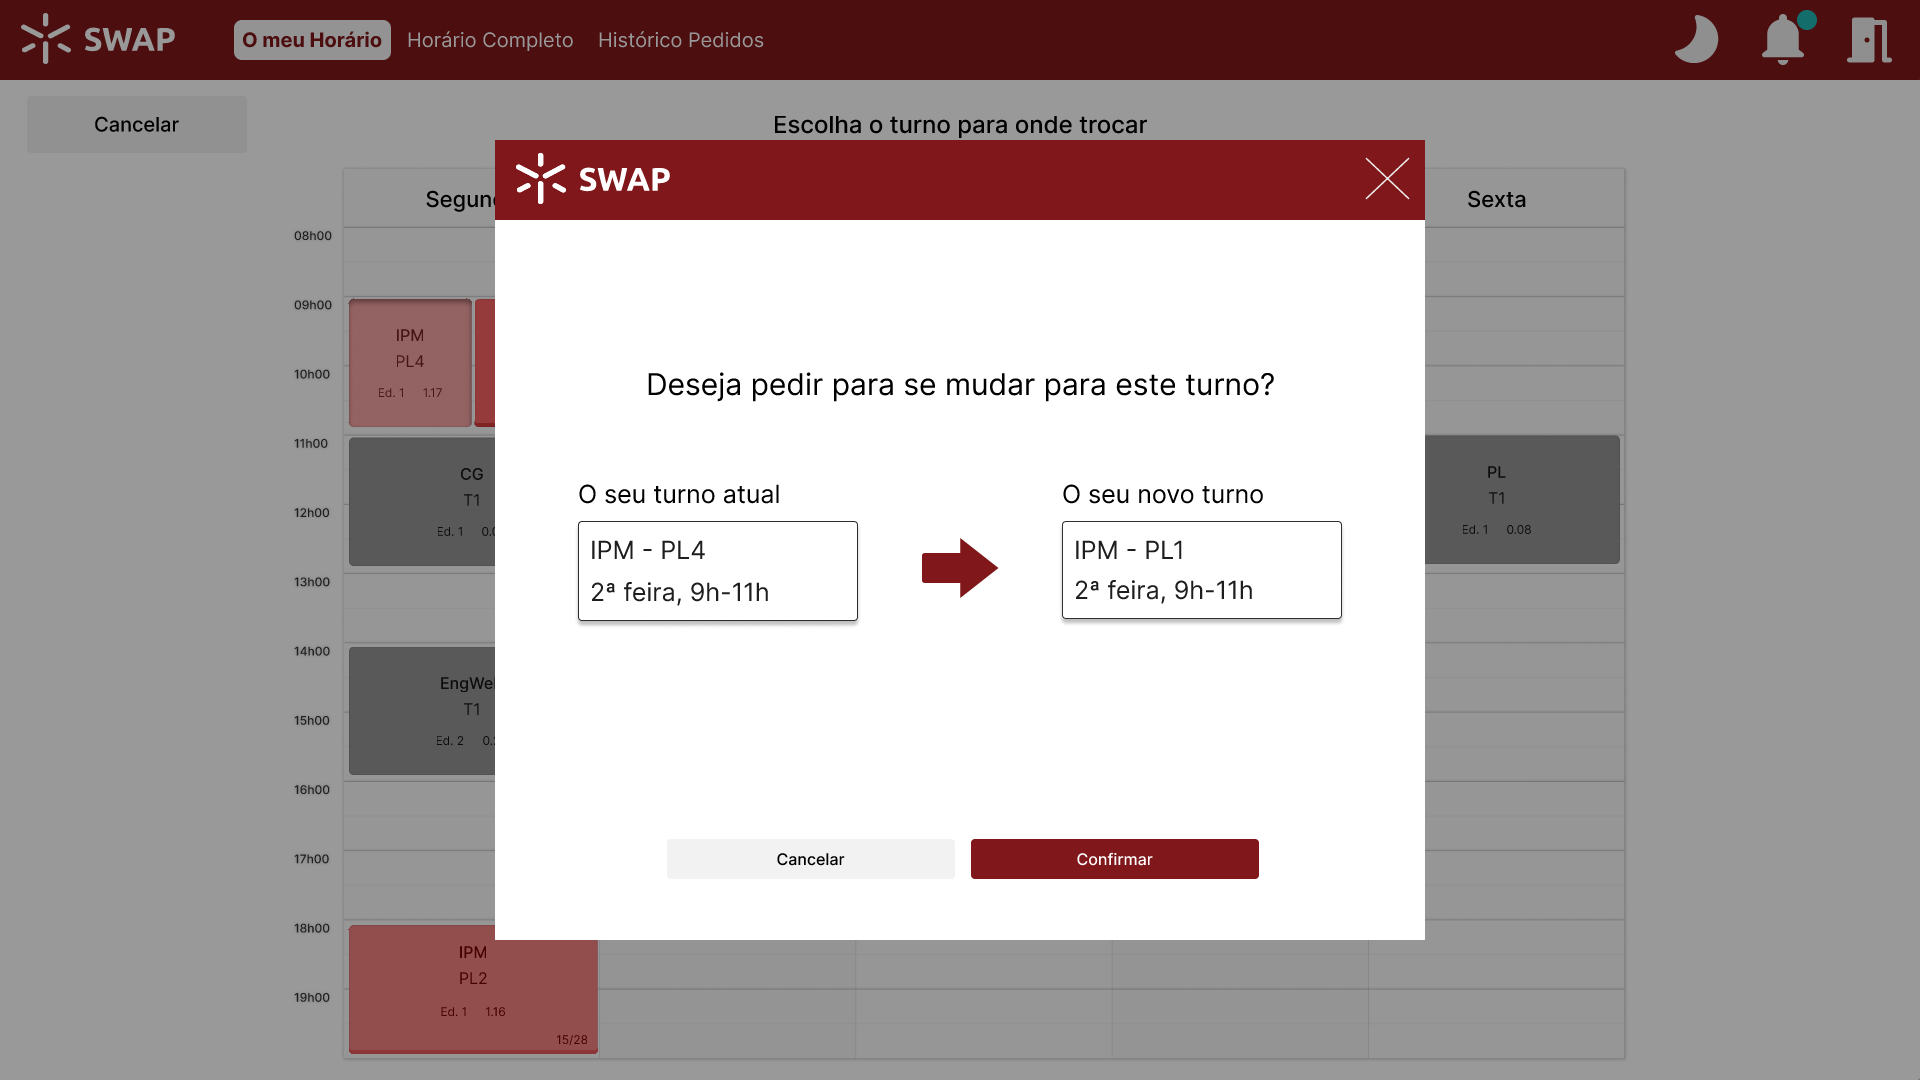
\includegraphics[width=0.8\textwidth]{res/prototype/dialogo-confirmacao-troca.png}
    \caption{Diálogo para confirmação da troca de um turno na página ``O meu Horário''.}
    \label{dialogo-confirmacao-troca}
\end{figure}

Caso o utilizador cancele a troca ou feche este diálogo, voltará à vista da página para escolha
escolha de turnos da figura \ref{o-meu-horario-trocar}. Caso confirme a troca, o utilizador será
redirecionado para o vista inicial da página ``O meu Horário'', com uma mensagem a mostrar que o
pedido de troca foi enviado. Este \emph{feedback} é especialmente importante para utilizadores menos
experientes, como os correspondentes ao perfil da Maria.

\begin{figure}[H]
    \centering
    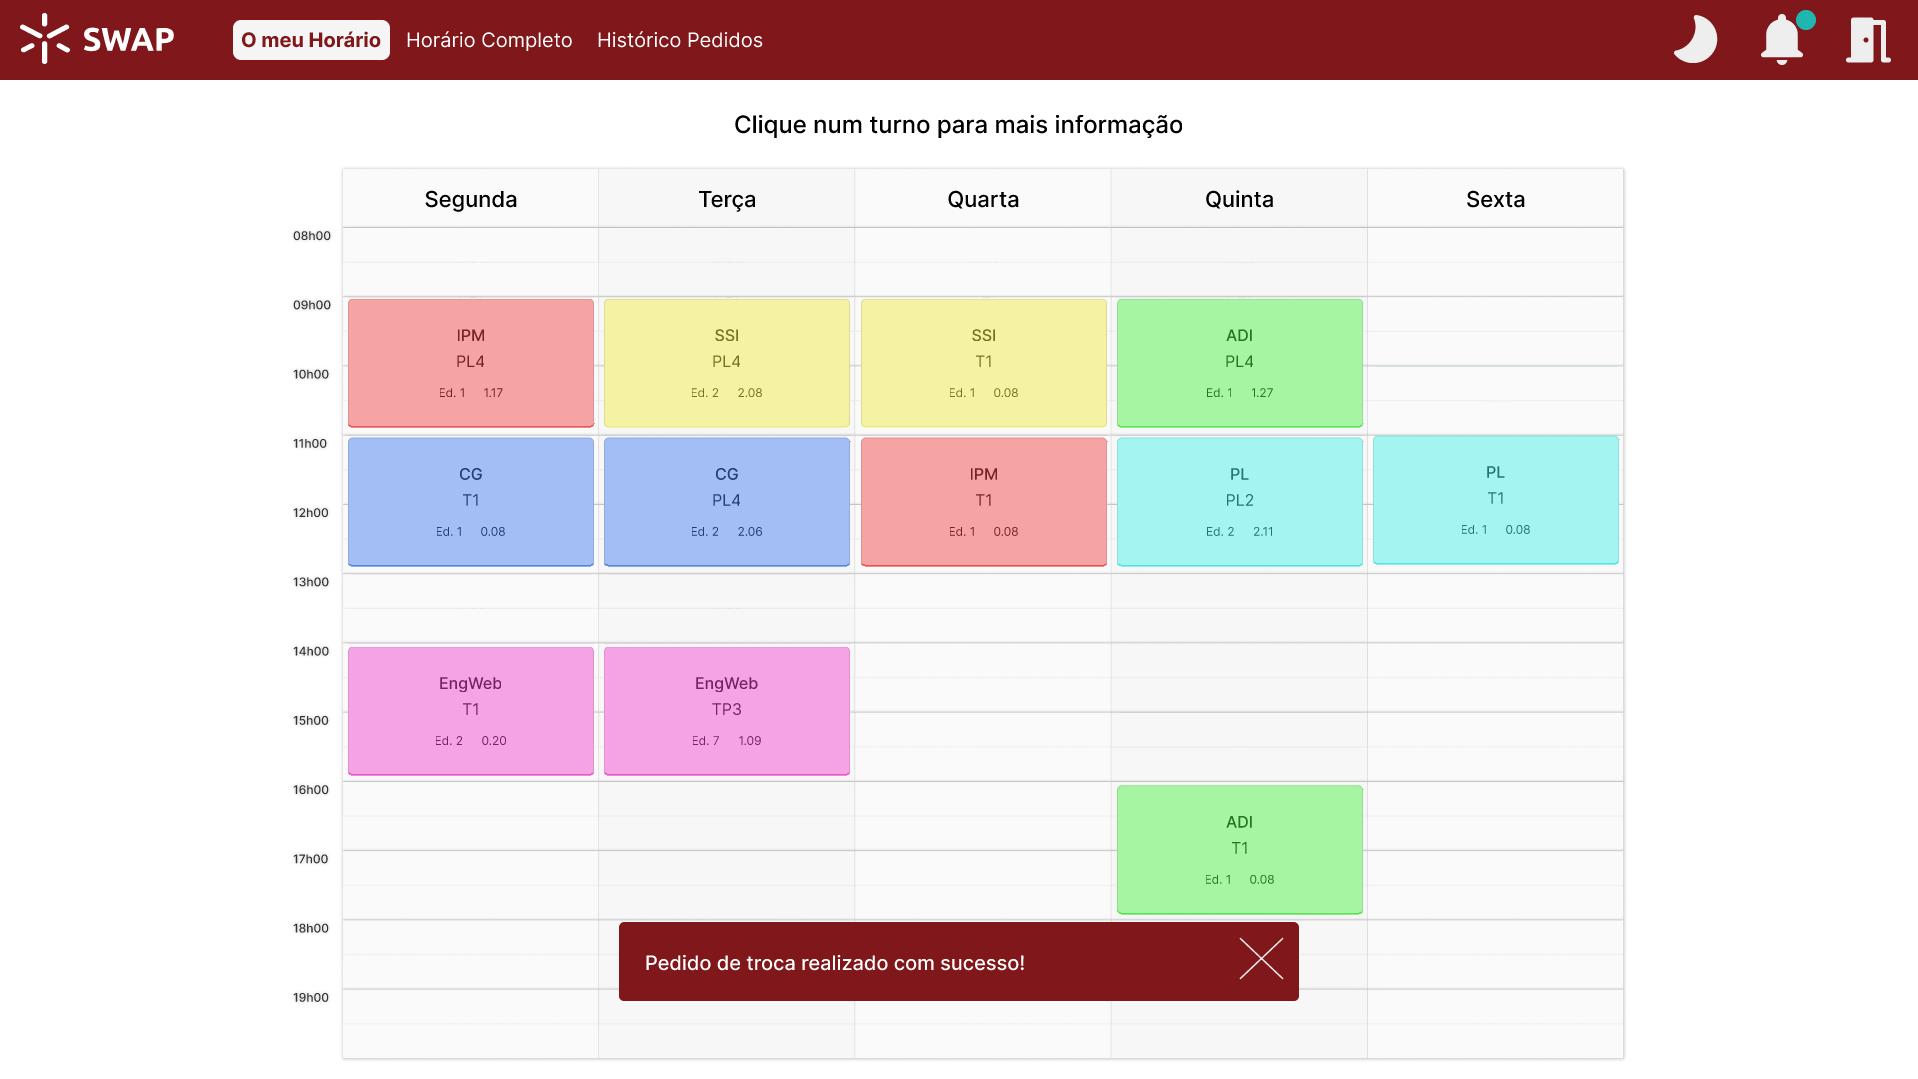
\includegraphics[width=0.8\textwidth]{res/prototype/o-meu-horario-toast-sucesso-troca.png}
    \caption{
        \onehalfspacing
        Captura de ecrã do protótipo da página ``O meu Horário'' com a confirmação de sucesso no
        envio de um pedido de troca de turno.
    }
    \label{o-meu-horario-toast-sucesso-troca}
\end{figure}

Esta mensagem deve desaparecer automaticamente após alguns segundos. No entanto, devido a limitações
do Figma, não foi possível incluir esta funcionalidade no protótipo.

\subsection{Página ``Horário Completo''}

A página ``O meu Horário'' é útil para alunos que procuram trocar apenas um turno: podem selecionar
o turno que desejam trocar, conhecer as alternativas disponíveis, e pedir para trocar para a que
mais lhes agrada. No entanto, se os alunos desejarem trocar mais do que um turno, podem querer ver
em simultâneo as várias possibilidades de troca dos vários turnos que desejam trocar. Caso a Maria
tenha mais do que uma aula na quinta de manhã, como descreve o cenário 4, poderá ter de trocar mais
do que um turno. Por este motivo, foi prototipada a página ``Horário Completo'', onde o utilizador
pode ver todos os turnos de todas as UCs em que se encontra inscrito:

\begin{figure}[H]
    \centering
    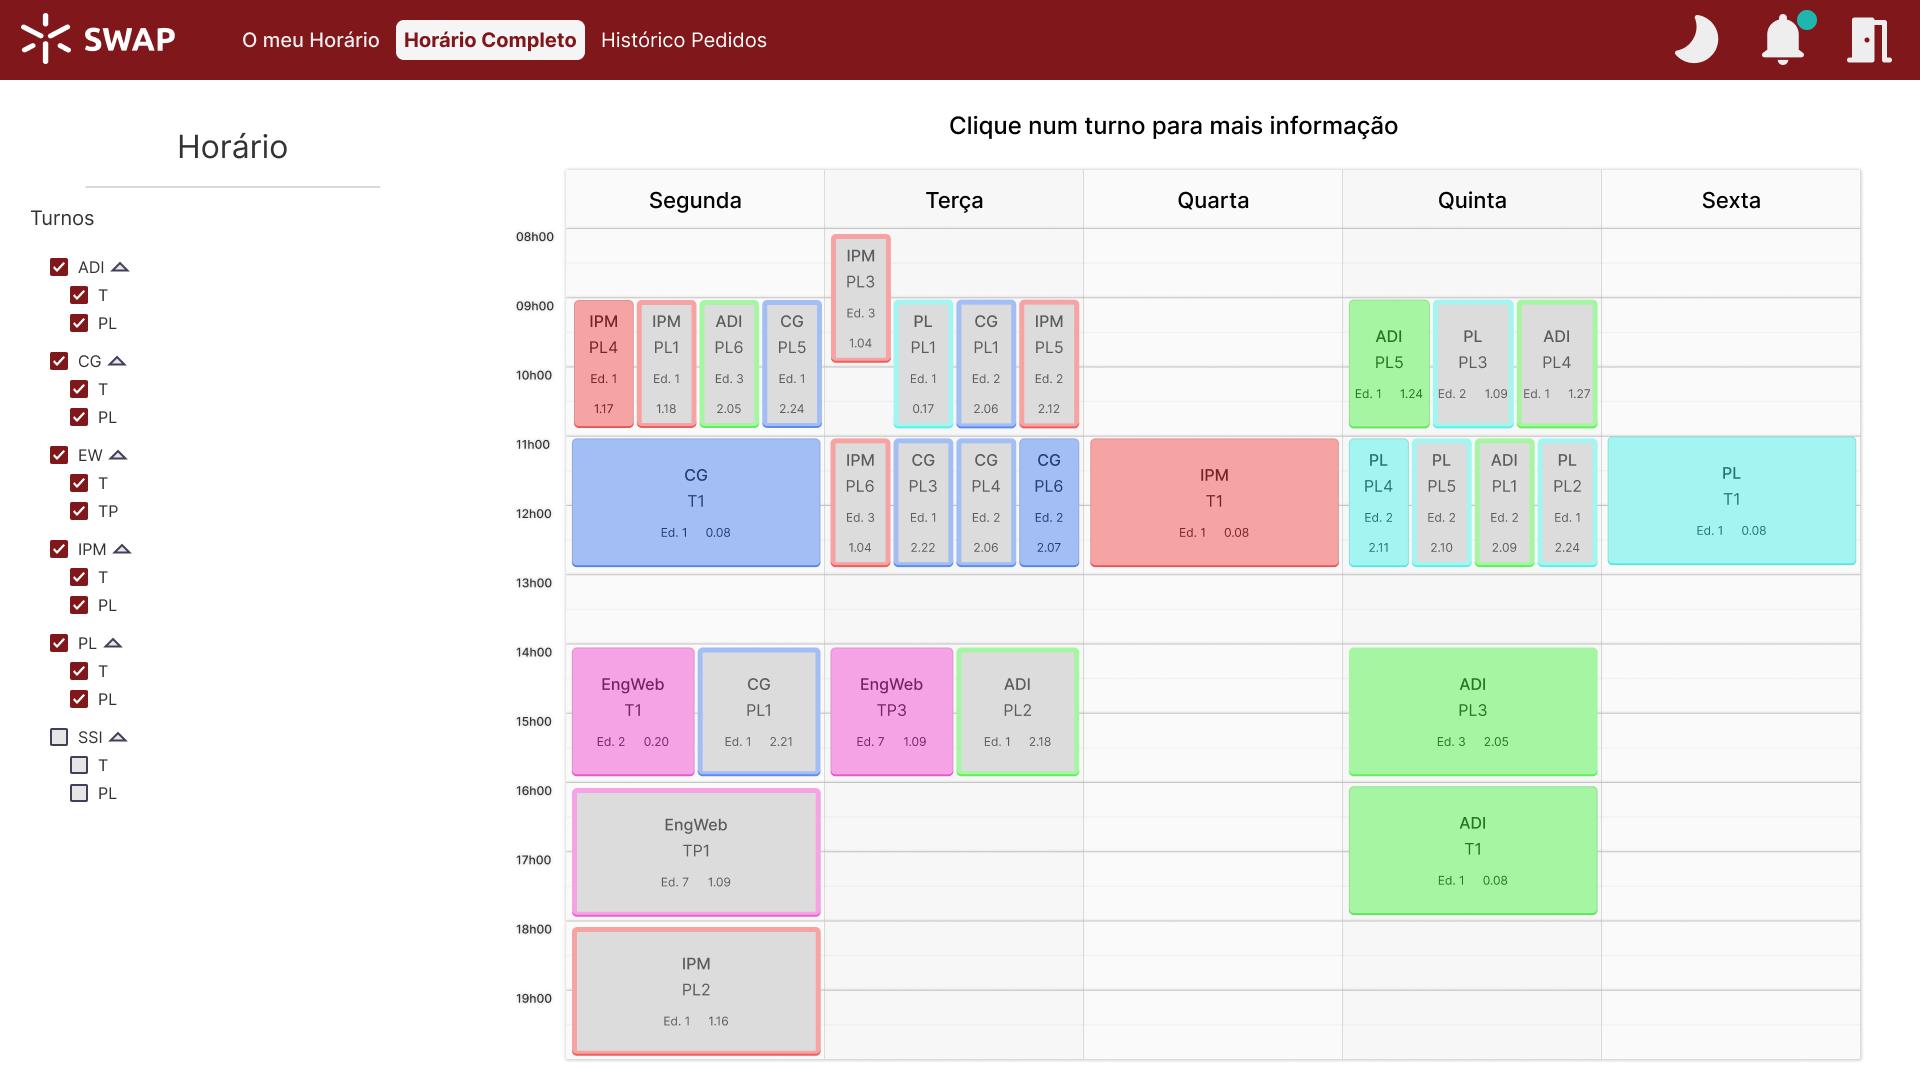
\includegraphics[width=0.8\textwidth]{res/prototype/horario-completo.png}
    \caption{
        \onehalfspacing
        Captura de ecrã do protótipo da página ``Horário Completo'' durante uma troca de turnos.
    }
    \label{horario-completo}
\end{figure}

Como se pode observar, os turnos em que o aluno se encontra inscrito são apresentados em tons
coloridos, realçando as horas em que o aluno não deve escolher novos turnos, pois fazê-lo poderá
conduzir a sobreposições. Os turnos em que o aluno não se encontra inscrito são apresentados a
cinzento, com uma borda da cor correspondente à sua UC. Deste modo, o utilizador pode facilmente,
com base numa cor, identificar todos os turnos associados a uma UC.

Como podem ser muitos os turnos de todas as UCs em que o aluno se encontra inscrito, foi adicionada
uma barra lateral à página, que permite ao utilizador escolher que turnos deseja que sejam
apresentados. Deste modo, a observabilidade da página é melhorada, especialmente em ecrãs mais
pequenos. Ademais, também é adicionada alguma costumizabilidade, visto que o utilizador é capaz de
escolher que informação lhe é apresentada, podendo optar, por exemplo, por ignorar turnos de UCs
que não deseja alterar.

Caso o utilizador clique num turno para o trocar, será aberto o diálogo apresentado na figura
\ref{dialogo-informacao-turno}, a partir do qual o utilizador poderá ir para a seguinte vista da
página ``Horário Completo'':

\begin{figure}[H]
    \centering
    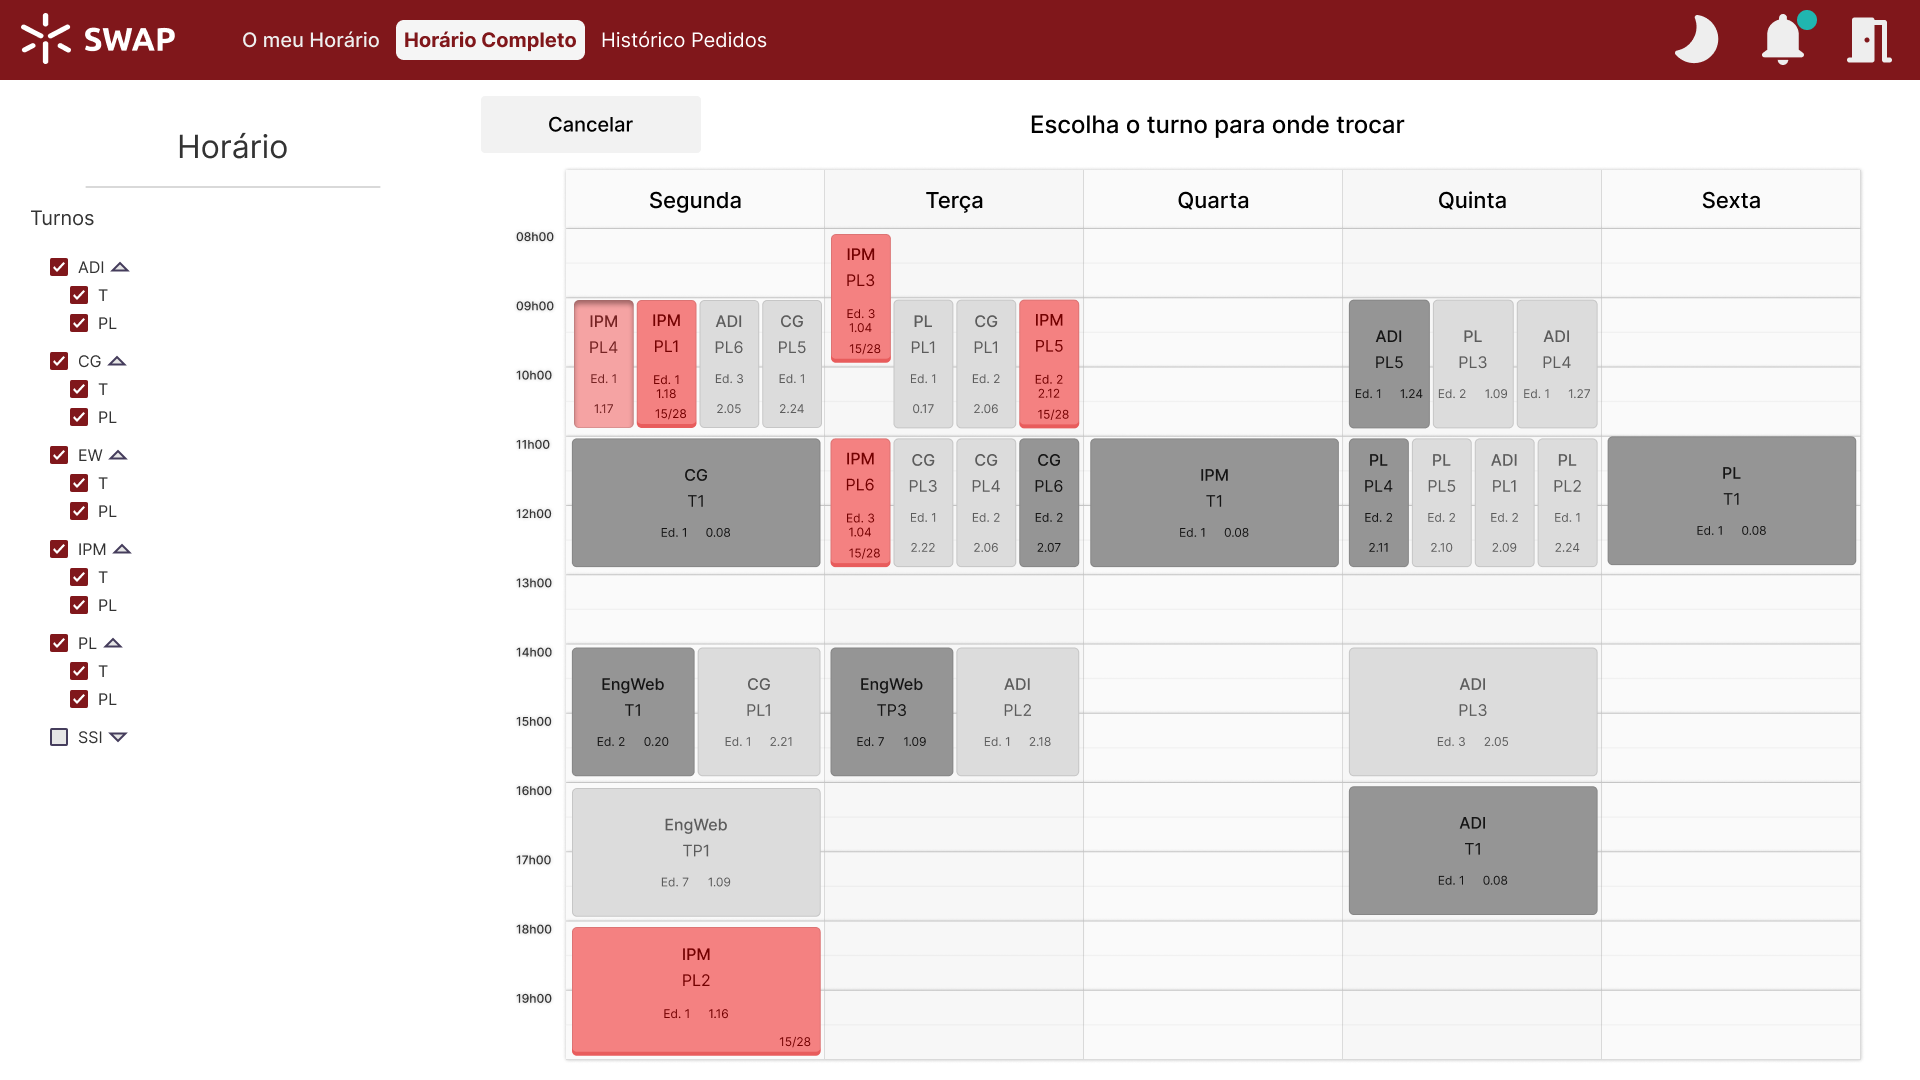
\includegraphics[width=0.8\textwidth]{res/prototype/horario-completo-trocar.png}
    \caption{Captura de ecrã do protótipo da página ``Horário Completo''.}
    \label{horario-completo-trocar}
\end{figure}

Esta vista da página ``Horário Completo'' foi modelada com base na vista apresentada na figura
\ref{o-meu-horario-trocar}. No entanto, de uma forma consistente com a vista normal da página
``Horário Completo'', mantém-se a barra lateral, onde o utilizador pode ajustar os turnos que deseja
ver no horário. Além disso, passa a haver uma distinção entre os tons de cinzento dos turnos com os
quais não é possível interagir: um cinzento mais escuro é utilizado para apresentar os turnos nos
quais o aluno se encontra inscrito, e um cinzento mais claro é usado para apresentar os restantes
turnos. Espera-se que este realce do horário atual do aluno o ajude a detetar possíveis
sobreposições resultantes da troca de um turno.

Quando o utilizador carrega num turno, a aplicação deve comportar-se do modo previamente descrito
para a página ``O meu Horário'': o diálogo apresentado na figura \ref{dialogo-confirmacao-troca}
deve aparecer e, caso o utilizador confirme a troca de turno, o estado da página deverá ser
reiniciado, e uma confirmação de envio do pedido deverá ser apresentado:

\begin{figure}[H]
    \centering
    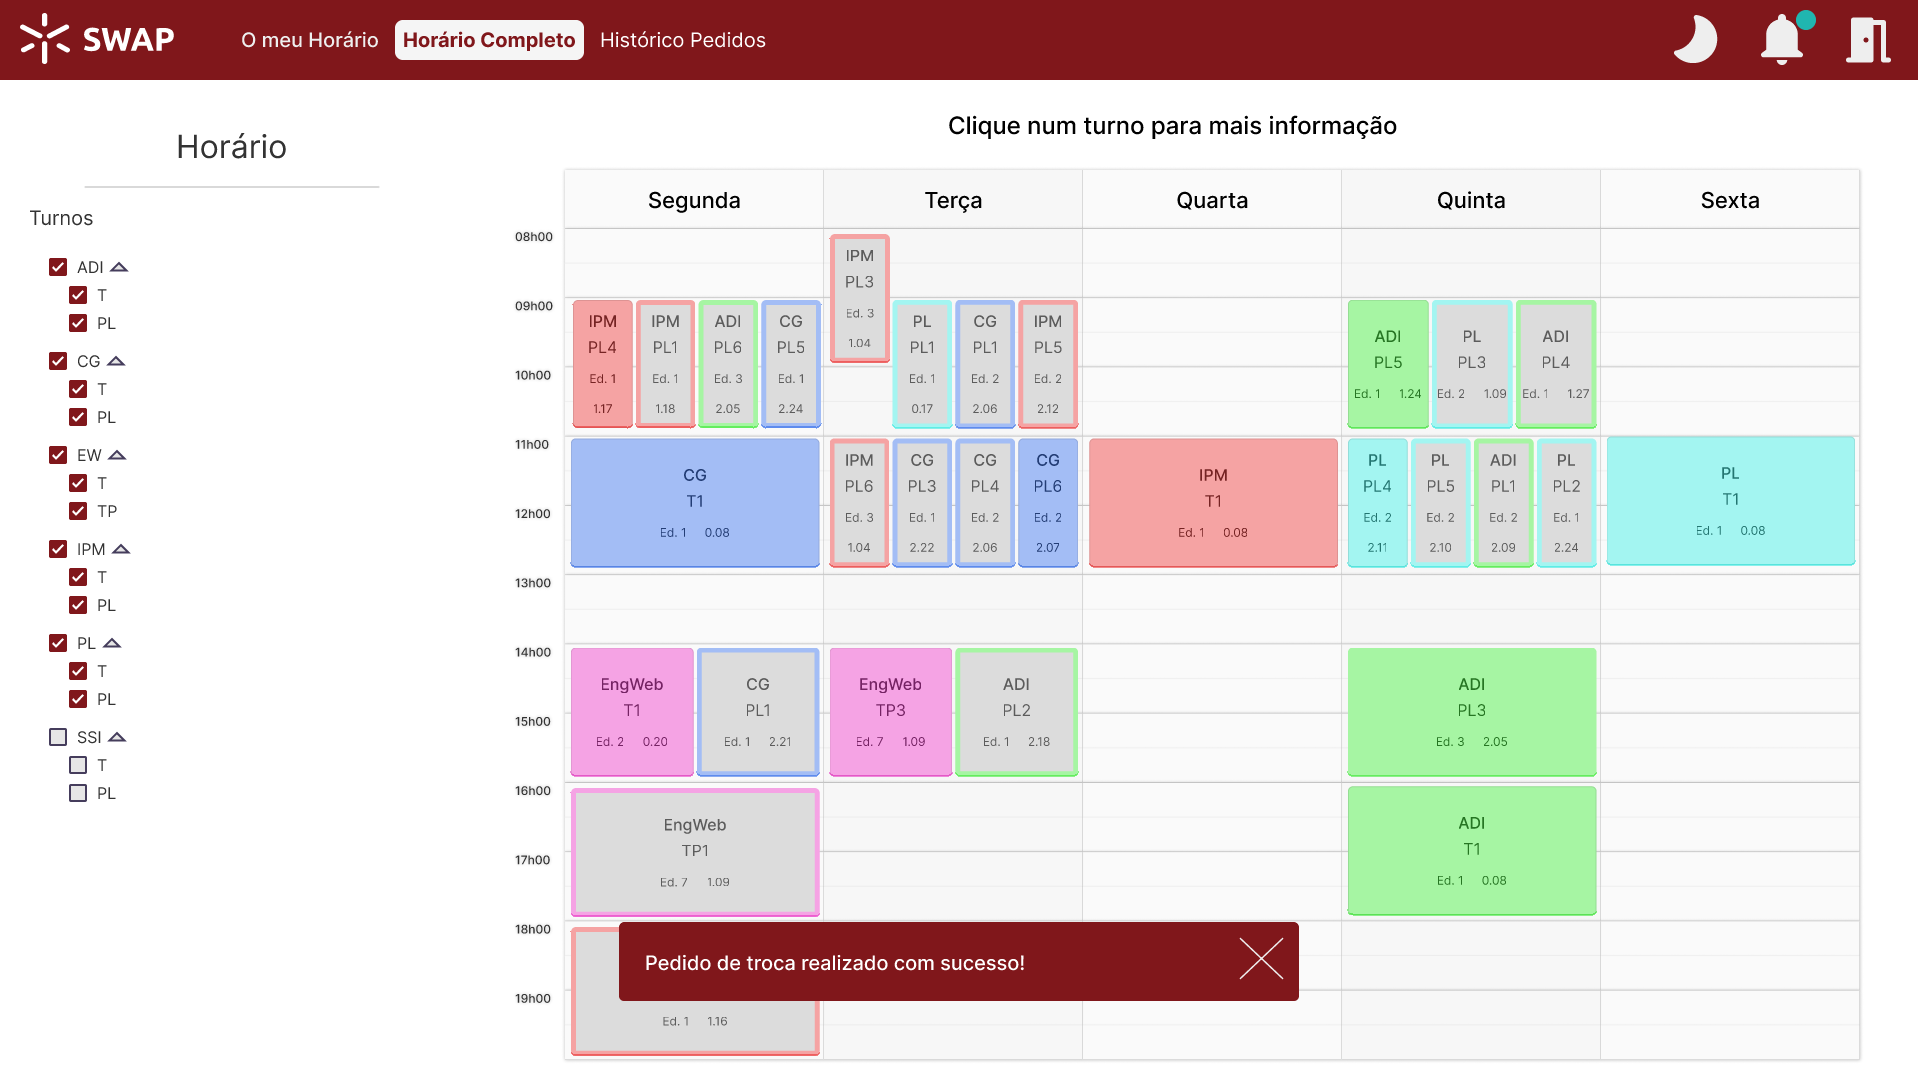
\includegraphics[width=0.8\textwidth]{res/prototype/horario-completo-toast-sucesso-troca.png}
    \caption{
        \onehalfspacing
        Captura de ecrã do protótipo da página ``Horário Completo'' com a confirmação de sucesso no
        envio de um pedido de troca de turno.
    }
    \label{horario-completo-toast-sucesso-troca}
\end{figure}

\subsection{Página ``Histórico de Pedidos''}

Foi criada uma página para apresentar ao utilizador os pedidos de troca de turnos que este fez no
passado. Esta não passa de uma lista dos pedidos, ordenados do mais recente para o mais antigo:

\begin{figure}[H]
    \centering
    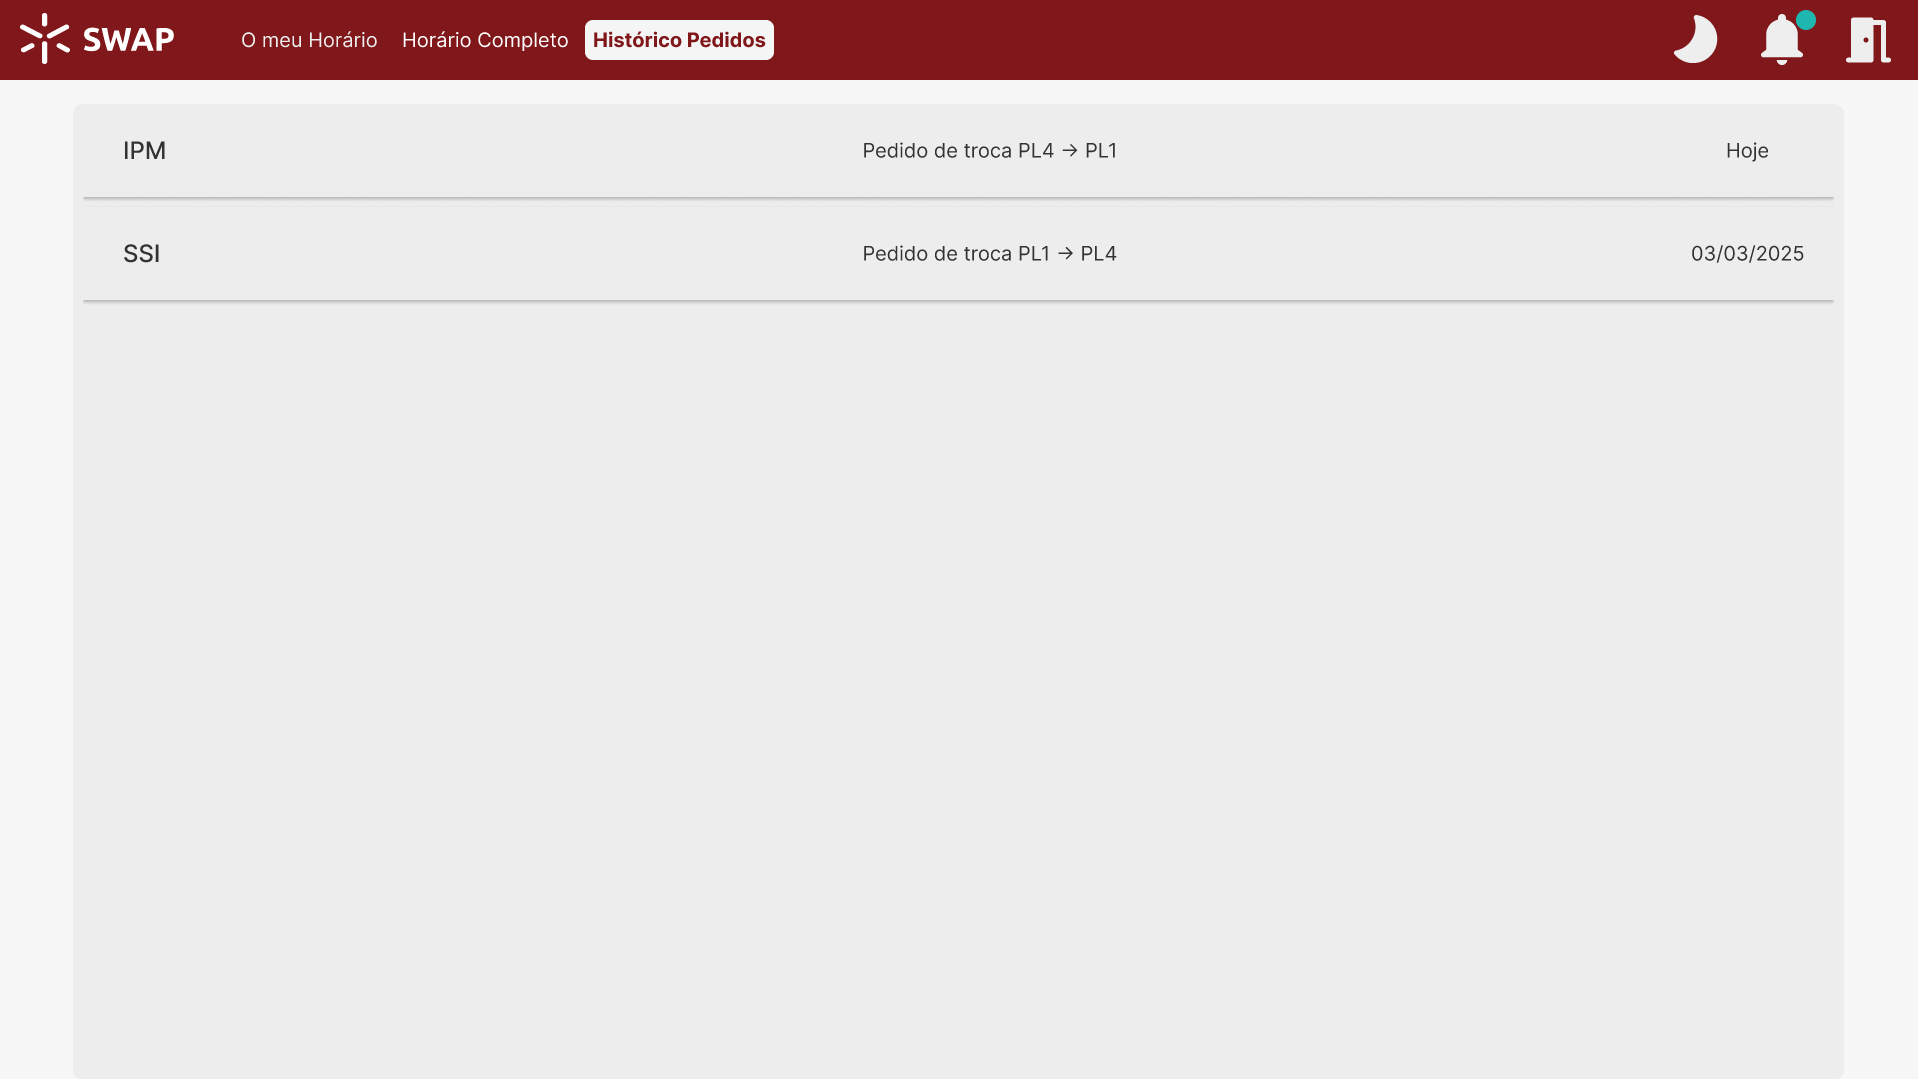
\includegraphics[width=0.8\textwidth]{res/prototype/historico-de-pedidos.png}
    \caption{Captura de ecrã do protótipo da página ``Histórico de Pedidos''.}
    \label{historico-de-pedidos}
\end{figure}

\subsection{Página ``Notificações do Aluno''}

Os alunos que utilizam a aplicação devem ter uma forma de serem notificados de eventos importantes.
Estas notificações podem ser consultadas na página cujo protótipo se apresenta abaixo, acessível
através do ícone com um sino na barra de navegação:

\begin{figure}[H]
    \centering
    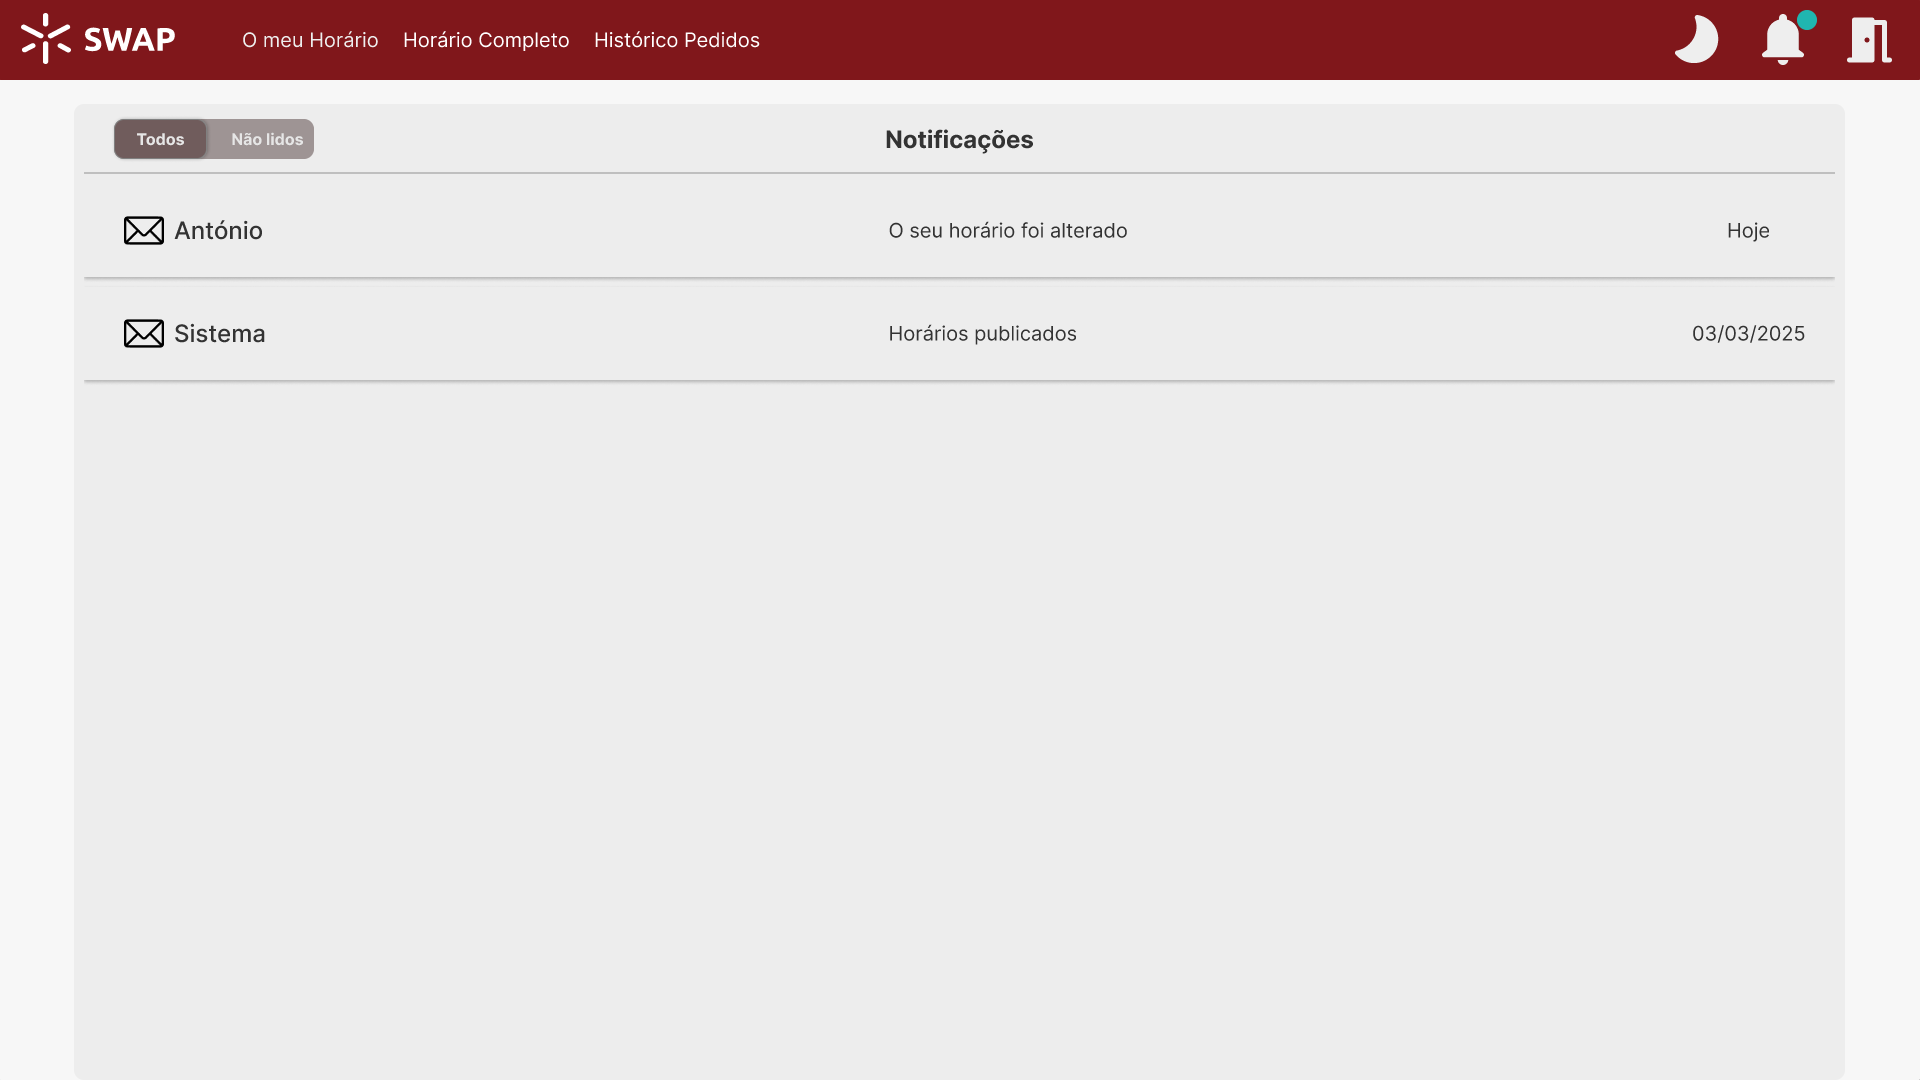
\includegraphics[width=0.8\textwidth]{res/prototype/notificacoes-aluno.png}
    \caption{Captura de ecrã do protótipo da página ``Notificações do Aluno''.}
    \label{notificacoes-aluno}
\end{figure}

Como se pode observar, esta página apresenta as notificações da mais recente para a mais antiga.
Adicionalmente, com o \emph{toggle} no canto superior esquerdo, é possível alternar entre a
apresentação de todas as notificações e apenas das notificações por ler. Ademais, como esta página
não é acessível a partir da barra de navegação, o seu título, ``Notificações'', não é realçado na
mesma, tendo de ser incluído nos seus conteúdos.

Por último, para uma boa experiência de utilização sem distrações desnecessárias, é importante que
as notificações sejam relevantes para o utilizador. Assim, definiram-se os seguintes tipos de
notificação:

\begin{itemize}
    \item Atribuição de um horário ao aluno, consequência da primeira publicação dos horários por
        parte do diretor de curso (cenário 1);
    \item Recusa de um pedido de mudança de turno pelo diretor de curso (cenário 3). Deste modo, o
        aluno sabe que o seu pedido não será satisfeito antes do diretor de curso publicar novos
        horário, fazendo com que possivelmente possa pedir para trocar outros turnos;
    \item Atualização do horário do aluno (cenário 3), que ocorre quando o diretor de curso publica
        novos horários e o conjunto de turnos que o aluno deve frequentar é alterado.
\end{itemize}

\section{Mapa de Navegação}

\section{Avaliação Heurística}

\section{Conclusão e Trabalho Futuro}

\begingroup
\section{Bibliografia}
\renewcommand{\section}[2]{}

\begin{thebibliography}{9}
    \bibitem{figma}
        "Figma: Collaborative Interface Design Tool."{}. Figma. Accessed: Mar. 13, 2025. [Online.]
        Available: \url{https://www.figma.com/}
    \bibitem{nielsen}
        "10 Usability Heuristics for User Interface Design". Nielsen Norman Group.
        Accessed: Mar. 13, 2025. [Online.] Available:
        \url{https://www.nngroup.com/articles/ten-usability-heuristics/}
    \bibitem{material-icons}
        "Material Symbols \& Icons"{}. Google Fonts. Accessed: Mar. 14, 2025. [Online.] Available:
        \url{https://fonts.google.com/icons}
\end{thebibliography}
\endgroup

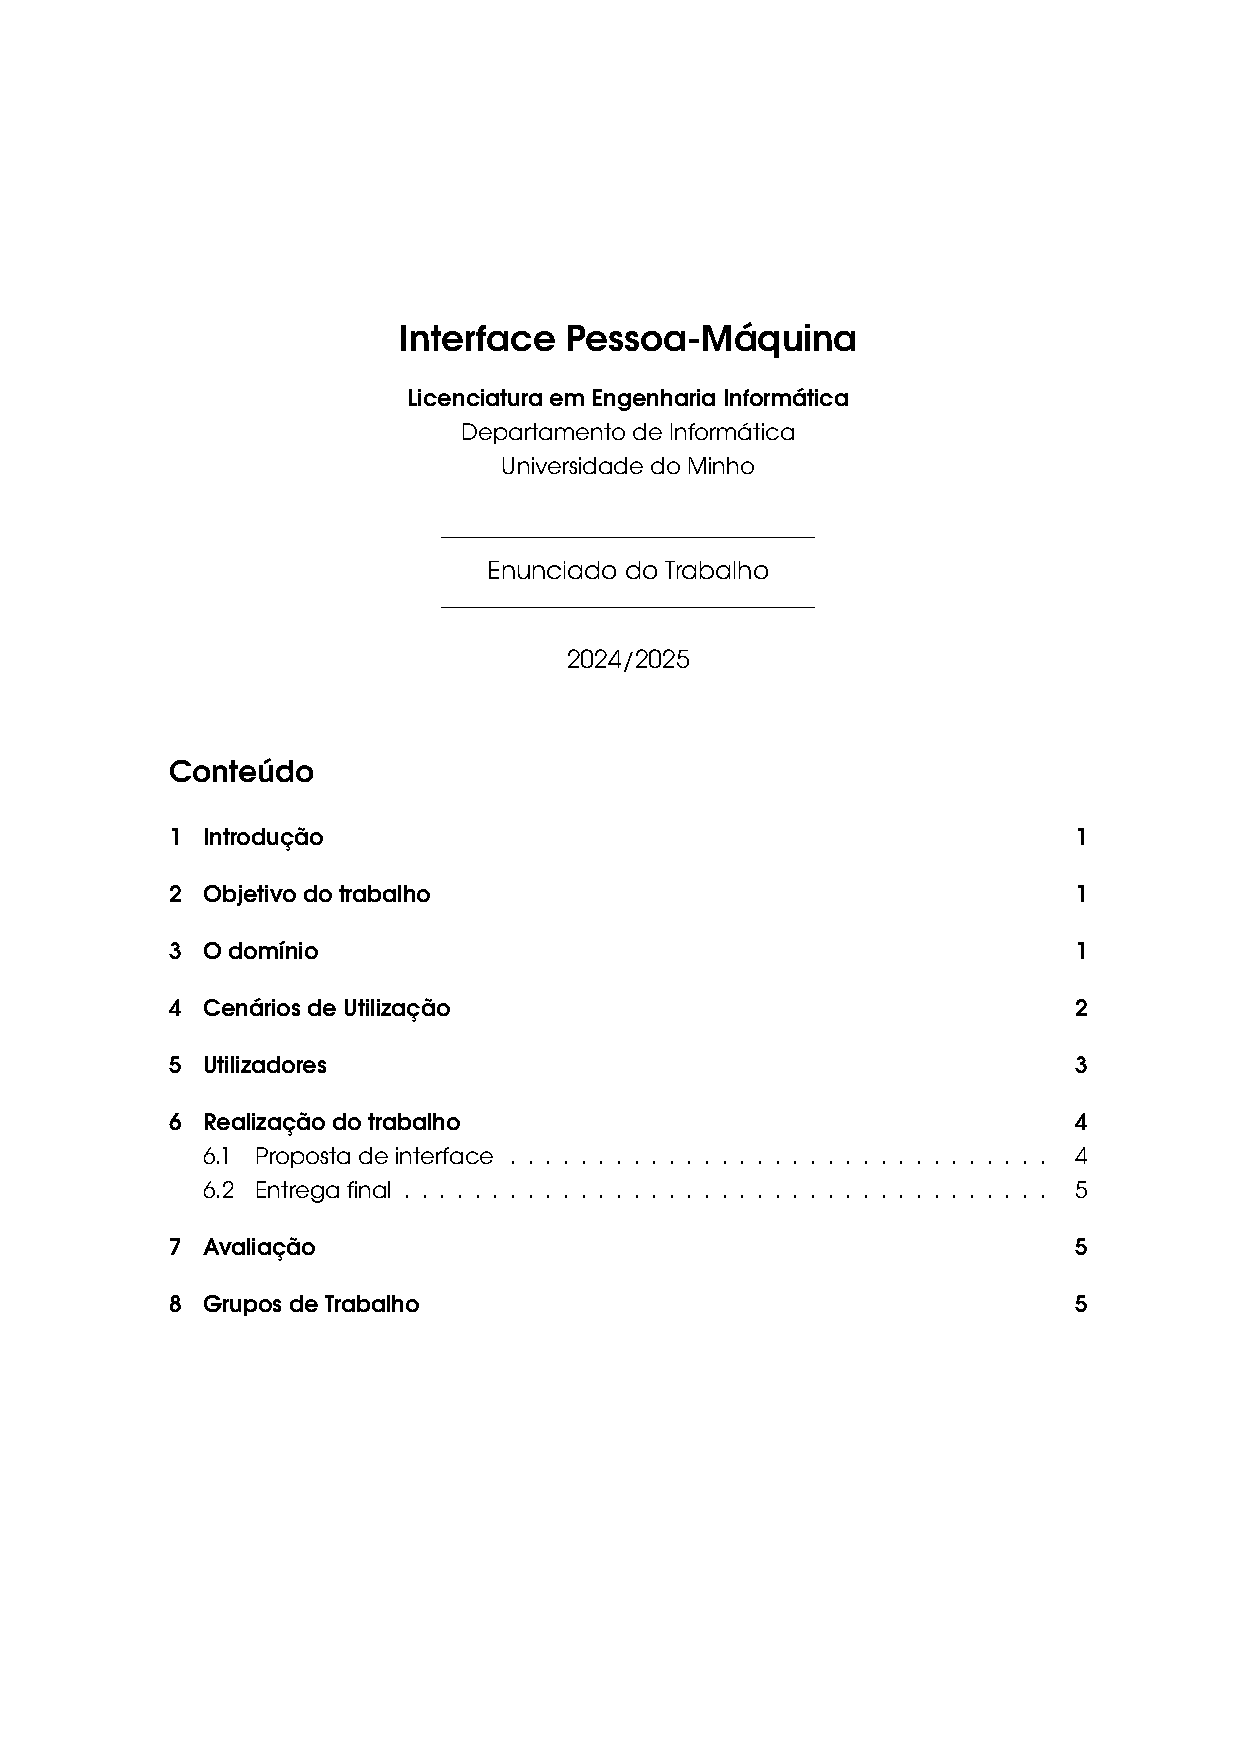
\includepdf[pages=1,pagecommand=\section{Anexo -- Enunciado do Trabalho}\thispagestyle{empty}]
    {../Assignment.pdf}
\includepdf[pages=2-]{../Assignment.pdf}

\end{document}
